\chapter{Oil, Gas, and the Structure of Industrial Wealth}

These notes, drawn from a School of Hard Knocks interview and curated by LazyingArt LLC, follow a field-level investigation of oil and gas as a machine for creating wealth. The lecture does not begin with a commodity graph or a legal treatise. It begins with a provocation: oil and gas may have created more durable fortunes than the sectors that command fashionable attention. From there we are taken to El Campo, Texas, to a live rig, to the control room, and only then to the deeper structure of the business: distressed asset purchase, day-rate economics, monitored drilling, lease terms, royalty claims, and the split between mineral ownership and working-interest exposure. We will keep that order, because the argument unfolds by successive clarification.

\section{The Hidden Wealth Machine in the Field}

The lecture opens with scale before detail. Oil and gas is introduced as an industry that has built dynasties, powered nations, and continued to mint large fortunes even while public attention drifts elsewhere. Then the rhetoric contracts sharply. We are no longer speaking about civilization in the abstract; we are in the Texas oil field, in the middle of nowhere, standing near a live rig.

That movement matters. The host does not promise a generic success story. He promises a masterclass in a business he himself finds unfamiliar. He says, in effect: we are going straight to the source; we will walk the rigs; we will ask how the money is made; and we will ask whether the returns can in fact outrun the stock market or real estate. The lecture's first real question is therefore not ``what is oil?'' but rather: why does this industry look so obscure from the outside if its wealth effects are so large on the inside?

Even at the outset one can see that the lecture treats oil and gas not as a single market, but as a layered system. There is a physical layer of rigs, wells, pipe, and monitoring. There is a legal layer of title, lease, royalty, and working interest. And there is a financial layer of distressed acquisition, fund structure, and investor participation. The lecture's value lies in showing how these layers lock together.

\section{From Roughneck Labor to an Integrated Oil Business}

Brent Franklin's biography arrives early because the lecture wants to remove some of the mystique from entry into the field. He describes himself as mowing grass after leaving the Navy, receiving a call from a friend in Midland--Odessa, taking a job on an oil rig, and then, within a few years, buying rigs of his own. The biographical point is not romance. It is structural. In this industry, knowledge is tied to machinery, repetition, danger, and time spent inside the work.

The lecture then supplies scale. Brent says that the company did about
\begin{equation}
R_{\mathrm{year}} \approx 40 \times 10^6\ \mathrm{USD}
\end{equation}
in the last year across all of its platforms. The phrase ``across all of its platforms'' is crucial. He does not present the business as a single well or a single lucky strike. He presents it as an integrated stack: buying distressed off-market oil-and-gas properties, fixing them, drilling wells, repairing wells, and building an investment structure through which outside capital can participate without itself becoming an operating company.

This is the lecture's first serious economic clarification. From a distance, one imagines oil wealth as a gush of commodity revenue. At field level, however, the business is more intricate. It can include service income, asset acquisition below replacement cost, operational turnaround, lease economics, and capital structuring. The glamour of the commodity sits on top of a less glamorous but far more intelligible arrangement of machines and contracts.

\begin{table}[h]
\centering
\begin{tabular}{|l|l|}
\hline
Quantity & Value reported in the lecture \\
\hline
Annual business scale & \(R_{\mathrm{year}} \approx 40 \times 10^6\ \mathrm{USD}\) \\
Rig day rate & \(R_{\mathrm{day}} = 15{,}500\ \mathrm{USD/day}\) \\
Replacement cost of rig & \(C_{\mathrm{new}} \approx 6.5 \times 10^6\ \mathrm{USD}\) \\
Purchase basis & about \(15\%\) of replacement cost \\
Whole depth on monitor & \(D = 4599.5\ \mathrm{ft}\) \\
Starter capital benchmark & \(K_0 \approx \$100{,}000\) \\
Rig specification & top-drive rig, about \(850\) horsepower \\
\hline
\end{tabular}
\caption{Quantitative markers carried explicitly by the lecture.}
\end{table}

The arithmetic of distressed acquisition is one of the cleanest pieces of mathematics in the lecture. Brent says that a new version of the rig on site would cost about
\begin{equation}
C_{\mathrm{new}} \approx 6.5 \times 10^6\ \mathrm{USD},
\end{equation}
while his company bought the actual rig for about fifteen cents on the dollar:
\begin{equation}
C_{\mathrm{buy}} \approx 0.15\,C_{\mathrm{new}} \approx 0.15 \times 6.5 \times 10^6 \approx 9.75 \times 10^5\ \mathrm{USD}.
\end{equation}
He adds that the prior owner had paid over five million dollars for the same piece of equipment. The point is not merely that bankruptcy creates bargains. It is that industrial wealth can begin with replacement-cost asymmetry. If one can buy operating equipment far below new-build cost, then one enters the same field with a very different basis.

\paragraph{Worked example.} The acquisition logic can be written in four short steps:
\begin{enumerate}
\item Begin with the reported replacement benchmark \(C_{\mathrm{new}} \approx 6.5 \times 10^6\ \mathrm{USD}\).
\item Apply the stated distress discount \(C_{\mathrm{buy}} \approx 0.15\,C_{\mathrm{new}}\).
\item Compute the implied purchase basis:
\[
C_{\mathrm{buy}} \approx 9.75 \times 10^5\ \mathrm{USD}.
\]
\item Read the spread not as paper profit, but as room to operate a service machine under inherited contracts and daily billing.
\end{enumerate}

Already we can see the chapter's first serious theme. Oil wealth is not only about what comes out of the ground. It is also about when assets are bought, from whom, and under what stress.

\section{Why Oil Makes Fortunes and Eats Fortunes}

Immediately after the wealth claim comes the correction. Brent gives the old oil-field line: if one wants to make a small fortune in oil and gas, one should start with a large fortune. That is not an aside. It is the lecture's first attempt to separate myth from operating truth.

The lecture insists on three conditions: consistency, diversification, and risk tolerance. Here the notes should slow down. Oil and gas is not presented as a lottery ticket. It is presented as a field in which fortunes are made by surviving volatility, buying correctly, structuring correctly, and not concentrating all one's exposure in a single fragile bet.

This is also where Brent introduces a second important beat that later governs the investment discussion. He says that he came into the field as an investor, took losses, was promised dreams by promoters, and finally concluded that money does not come from chasing money. It comes from chasing problems and monetizing the solution to those problems. In other words, the profitable structure is not an accident. It is a response to repeated failure modes already present in the industry.

\subsection{Question \& Answer}

\paragraph{Question.} If oil and gas makes people rich, why do so many people lose money in it?

\paragraph{Answer.} Because the lecture's idea of wealth here is structural rather than magical. A single well can fail. A property can be overleveraged. A promoter can oversell the opportunity. An investor can misunderstand the legal form of the deal. And an otherwise promising project can still be ruined by concentration in the wrong operator or the wrong moment. The lecture therefore draws a hard distinction between \emph{participating in upside} and \emph{surviving downside}.

That distinction appears again when Brent advises that even a meaningful initial amount of capital should not be placed all at once into one well, one new drill, or one company. If we let the outsider's starting capital be
\begin{equation}
K_0 \approx \$100{,}000,
\end{equation}
then the disciplined pattern is not
\[
K_1 = K_0
\]
for a single exposure, but rather a partition,
\begin{equation}
K_0 = \sum_{i=1}^{n} K_i,
\end{equation}
across multiple wells, operators, or deal structures. The lecture's language is careful here: there may be no way to abolish risk, but there may be a way to mitigate loss.

The broader lesson is that oil and gas punishes conceptual laziness. One must know what one owns, how one gets paid, where the losses can fall, and what operational competence stands behind the offering. Only then can the industry be discussed as a wealth machine.

\section{The Rig as a 24/7 Business Machine}

Having corrected the fantasy of easy riches, the lecture walks us into the machine itself. We are shown the camp house, introduced to the tool pusher, and told that drilling is a \(24\)-hour operation. This is not color. It means that the business cannot be understood as the work of a lone proprietor. It requires shift continuity, supervision, procedural discipline, and what Brent calls an army of experienced people.

The operational point is reinforced by the safety discussion. The lecture points to fire-retardant clothing, sharp and heavy moving parts, and the danger of live industrial equipment. It also explains that on some sites one would carry an H$_2$S monitor, though not on this particular well because the wellbore is sealed and the dangerous gas is not present. Here the lecture performs one of its most useful conceptual reversals: the public sees ``black gold and money,'' but the operator sees weight, motion, exposure, and the need for control.

This is also where the lecture asks whether it is too late to enter the business. Brent's answer is that the present may be the right time precisely because the field is short of capital and because many old-style conventional rigs have disappeared. The opportunity, in his telling, comes not from ease but from thinning competition. That is an important motivation for the rest of the chapter: we are looking not at a frictionless boom, but at a capital-starved industrial niche.

After a short promotional detour, the lecture repairs the reader's orientation by making an elementary but indispensable distinction: a rig is not a well.

\begin{definition}
In the language of the lecture, a \emph{drilling rig} is the service machine that drills or services the hole, while a \emph{well} is the drilled asset itself. Owning the former is exposure to day-rate service income; owning the latter is exposure to production and to the legal structure of the lease.
\end{definition}

The rig on site is described as an \(850\)-horsepower top-drive drilling rig. Its first economics are therefore service economics, not yet production economics:
\begin{equation}
R_{\mathrm{day}} = 15{,}500\ \mathrm{USD/day}.
\end{equation}
If one writes the usual annualization with utilization \(u \in [0,1]\), then
\begin{equation}
R_{\mathrm{rig,annual}} = 365\,u\,R_{\mathrm{day}}.
\end{equation}
This is not a claim about realized yearly revenue for this specific rig. It is the bookkeeping identity hidden inside the lecture's story: a service machine bought below replacement cost can be monetized through daily operation under contract.

\begin{figure}[h]
\centering
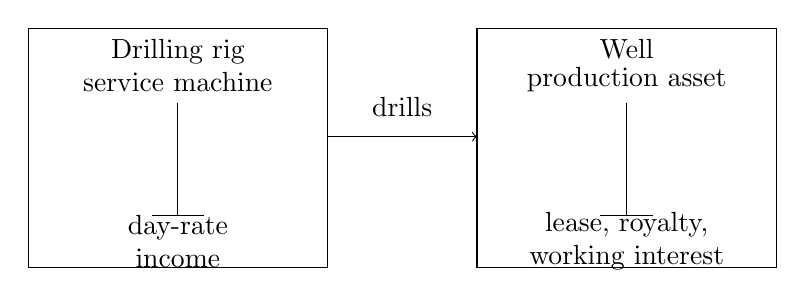
\begin{tikzpicture}[scale=0.95]
\draw (-5,1.6) rectangle (-1,-1.6);
\node at (-3,1.1) {\shortstack{Drilling rig\\service machine}};
\draw (-3,0.6)--(-3,-0.9);
\draw (-3.35,-0.9)--(-2.65,-0.9);
\node at (-3,-1.25) {\shortstack{day-rate\\income}};

\draw (1,1.6) rectangle (5,-1.6);
\node at (3,1.1) {\shortstack{Well\\production asset}};
\draw (3,0.6)--(3,-0.9);
\draw (2.65,-0.9)--(3.35,-0.9);
\node at (3,-1.25) {\shortstack{lease, royalty,\\working interest}};

\draw[->] (-1,0.15)--(1,0.15);
\node at (0,0.55) {drills};
\end{tikzpicture}
\caption{Transcript-derived schematic. The lecture insists that a rig is the machine that drills, while a well is the asset whose later economics are governed by lease terms and production rights.}
\end{figure}

But even after we know what the machine is, we still do not know what is happening below us. That is why the lecture next pauses inside the doghouse.

\section{The Doghouse, the Hole, and the Electronic Eyes of the Rig}

The doghouse is the closest thing this lecture has to a blackboard. Brent points to the PaceOn system and explains that it functions as the rig's electronic eyes and ears. It tells the crew the whole depth of the hole, where the bit is, what operation is currently underway, and what formations or gas signatures are being encountered.

The lecture gives one definite numerical reading:
\begin{equation}
D = 4599.5\ \mathrm{ft},
\end{equation}
and one definite operational reading: the rig is ``tripping.'' In cautious standard notation we may write
\begin{equation}
s \in \{\text{drilling},\ \text{tripping in},\ \text{tripping out}\}, \qquad s=\text{tripping}.
\end{equation}
Here tripping means that the crew is moving pipe in or out of the hole by assembling or removing joints rather than simply cutting new depth. The point is not the symbolism by itself. The point is that the monitor converts hidden motion underground into a state that can be read, communicated, and acted upon.

The lecture also stresses that the system is not merely a depth gauge. It reports formation information and gas information. One sees, not the rock directly, but a structured readout of the hole: depth, bit position, current operation, and the character of the material being traversed. In this sense, modern drilling is no longer blind, though it remains dangerous.

\begin{figure}[h]
\centering
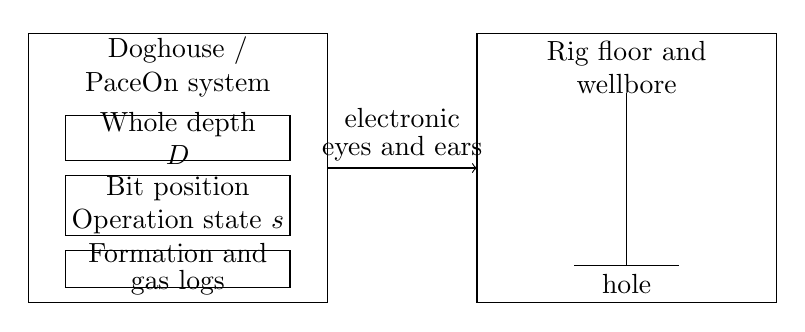
\begin{tikzpicture}[scale=0.95]
\draw (-5,1.8) rectangle (-1,-1.8);
\node at (-3,1.35) {\shortstack{Doghouse /\\PaceOn system}};
\draw (-4.5,0.7) rectangle (-1.5,0.1);
\node at (-3,0.4) {\shortstack{Whole depth\\\(D\)}};
\draw (-4.5,-0.1) rectangle (-1.5,-0.9);
\node at (-3,-0.5) {\shortstack{Bit position\\Operation state \(s\)}};
\draw (-4.5,-1.1) rectangle (-1.5,-1.6);
\node at (-3,-1.35) {\shortstack{Formation and\\gas logs}};

\draw (1,1.8) rectangle (5,-1.8);
\node at (3,1.35) {\shortstack{Rig floor and\\wellbore}};
\draw (3,1.0)--(3,-1.3);
\draw (2.3,-1.3)--(3.7,-1.3);
\node at (3,-1.55) {hole};

\draw[->] (-1,0)--(1,0);
\node at (0,0.45) {\shortstack{electronic\\eyes and ears}};
\end{tikzpicture}
\caption{Transcript-derived schematic of the operational picture. The floor itself is noisy and partially opaque; the doghouse converts motion in the hole into depth, bit position, state, and formation information.}
\end{figure}

\subsection{Question \& Answer}

\paragraph{Question.} If we cannot see into the well, what exactly does the driller know from the control room?

\paragraph{Answer.} He knows the hole indirectly but continuously. He does not see the subsurface as one sees a room. He sees an instrumented state: total depth, bit position, whether the crew is drilling or tripping, and the logs that indicate the formation and the possible appearance of gas. The lecture's point is not that technology removes danger. It is that modern drilling has replaced blindness with monitored interpretation.

From this point the lecture can return to the outsider's economic question. Once we know what the machine is doing, we can ask how someone who is not on the rig might participate in the business.

\section{How an Outsider Is Allowed to Invest}

The lecture returns now to a question that has been present from the beginning: if oil and gas is such a powerful wealth engine, how is an outsider supposed to enter? Brent's answer is restrictive rather than democratic. In one place he speaks of accredited investors; in another, of licensed investors. The legal phrasing is not fully stable in the lecture, but the practical point is clear enough: this is not being presented as a casual retail product.

The lecture gives three filters. First, one must meet the relevant gate for participation. Second, one must have substantial capital. Third, and most importantly, one must be able to bear total loss before entering the industry at all. The benchmark offered in the lecture is again
\begin{equation}
K_0 \approx \$100{,}000,
\end{equation}
but even this is not described as money to be placed all at once into one well, one new drill, or one company. The emphasis remains on dispersion and on the distinction between mitigating loss and pretending that risk has vanished.

The lecture also preserves the comparative frame introduced at the start. Brent says he has made money in real estate, likes real estate for long-term appreciation, and understands why the stock market attracts people. But he describes the stock market as a place where many nonprofessionals end up riding waves they do not know how to time. His conclusion is not that other assets are worthless. It is that intelligent investors diversify and partner with people who actually understand the game being played.

\begin{remark}
The lecture presents two strong claims here: first, that properly structured oil-and-gas investments may provide tax advantages against active income; second, that some deals can return more than \(100\%\) in less than a year. We record these as attributed claims about structure and operator quality, not as general guarantees of the asset class.
\end{remark}

If one compresses the second claim into mathematical shorthand, one obtains
\begin{equation}
\mathrm{ROI} > 100\%, \qquad t < 1\ \mathrm{year},
\end{equation}
or equivalently, if \(M\) denotes the capital multiple,
\begin{equation}
M>2, \qquad t < 1\ \mathrm{year}.
\end{equation}
But the lecture itself never treats these inequalities as independent truths. They are always tied to the phrase ``when structured properly.''

\subsection{Question \& Answer}

\paragraph{Question.} What does an outsider actually need in order to invest in oil and gas?

\paragraph{Answer.} In the lecture's account, the outsider needs more than money. He needs legal eligibility, enough capital to bear failure, and enough discipline not to treat a single deal as a destiny. He also needs operator judgment, either his own or someone else's. That is why Brent frames his company not merely as an owner of equipment, but as a structure built to solve the problems that uninformed investors encounter when they enter the field alone.

That last point is essential. The investment story in this lecture is not separable from the operational story. The whole argument is that understanding the machine changes what counts as a sensible financial claim.

\section{Rig, Well, Lease, Royalty, Working Interest}

This is the deepest and most useful section of the lecture. After discussing access to the industry, Brent turns to the structure of the industry itself. First comes the three-part chain:
\begin{equation}
\text{upstream} \longrightarrow \text{midstream} \longrightarrow \text{downstream}.
\end{equation}
Upstream refers to drilling and extraction. Midstream refers to movement and transport. Downstream refers to refining and finished products. This matters because the lecture explicitly corrects the naive idea that the operator simply ``sells gasoline.'' The path from hole to end product runs through several distinct businesses.

Then comes the rights split that most outsiders do not see. The person who owns the land at the surface need not own the minerals below it. Indeed, the lecture emphasizes that a tract may have many mineral owners. The landman enters precisely here: identifying title, assembling the area of interest, and negotiating the oil-and-gas lease.

From there we arrive at the lecture's main payout logic. Let \(G\) denote gross production revenue. If the royalty rate is
\begin{equation}
r = 25\% = 0.25,
\end{equation}
then the lecture's practical split is
\begin{align}
G &= rG + (1-r)G \\
  &= 0.25\,G + 0.75\,G.
\end{align}
The mineral-owner side receives the royalty share before expenses. The operator side receives the remainder. In the lecture's practical vocabulary, this mineral-owner gross share is also discussed through the label NRI. Thus if one is told that
\begin{equation}
\mathrm{NRI} = 20\% = 0.20,
\end{equation}
the lecture wants us to read
\begin{equation}
G = 0.20\,G + 0.80\,G,
\end{equation}
with the \(20\%\) going to the mineral-owner side and the \(80\%\) remaining on the operator side.

That remainder is then identified as the working-interest side, the side that actually bears drilling and operating costs. A cautious standard reconstruction is therefore
\begin{equation}
\Pi_{\mathrm{WI}} = (1-r)G - C_{\mathrm{drill}} - C_{\mathrm{op}},
\end{equation}
and if an investor purchases a fraction \(\alpha\) of that exposure, then
\begin{equation}
\Pi_{\alpha} = \alpha\,\Pi_{\mathrm{WI}} = \alpha\big((1-r)G - C_{\mathrm{drill}} - C_{\mathrm{op}}\big).
\end{equation}
This is not a formula written on the rig. It is the cleanest standard form of what Brent describes verbally: the investor pays into drilling, bears proportional cost, and receives proportional proceeds if the well is commercially productive.

\begin{figure}[h]
\centering
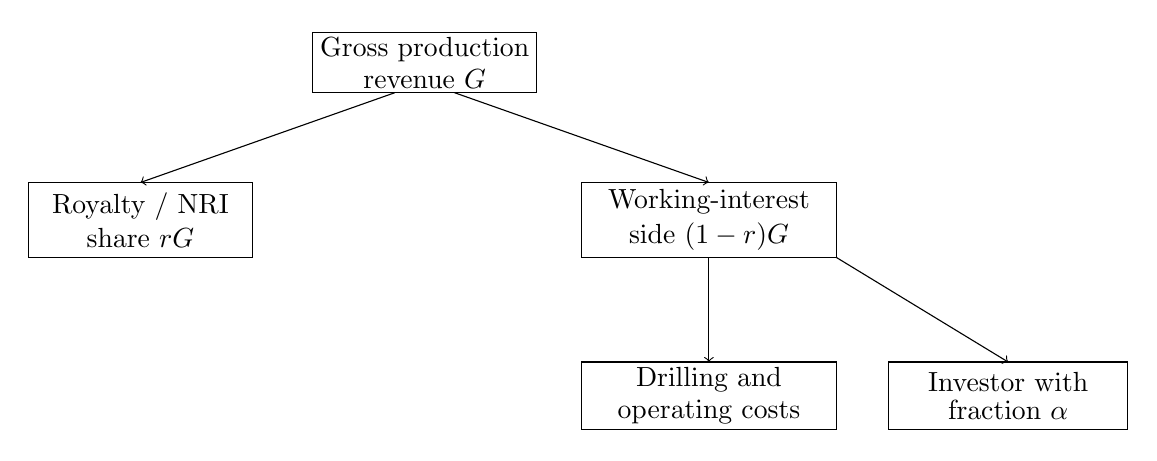
\begin{tikzpicture}[scale=0.95]
\draw (-1.4,3.0) rectangle (1.6,2.2);
\node at (0.1,2.6) {\shortstack{Gross production\\revenue \(G\)}};

\draw (-5.2,1.0) rectangle (-2.2,0.0);
\node at (-3.7,0.5) {\shortstack{Royalty / NRI\\share \(rG\)}};

\draw (2.2,1.0) rectangle (5.6,0.0);
\node at (3.9,0.5) {\shortstack{Working-interest\\side \((1-r)G\)}};

\draw[->] (-0.3,2.2)--(-3.7,1.0);
\draw[->] (0.5,2.2)--(3.9,1.0);

\draw (2.2,-1.4) rectangle (5.6,-2.3);
\node at (3.9,-1.85) {\shortstack{Drilling and\\operating costs}};

\draw (6.3,-1.4) rectangle (9.5,-2.3);
\node at (7.9,-1.85) {\shortstack{Investor with\\fraction \(\alpha\)}};

\draw[->] (3.9,0.0)--(3.9,-1.4);
\draw[->] (5.6,0.0)--(7.9,-1.4);
\end{tikzpicture}
\caption{Transcript-derived revenue and exposure schematic. In the lecture's practical presentation, gross revenue first splits between the mineral-owner share and the working-interest side; costs live on the working-interest side.}
\end{figure}

\subsection{Question \& Answer}

\paragraph{Question.} Who owns what, and who gets paid first when oil and gas is produced?

\paragraph{Answer.} The lecture's answer is layered. Surface ownership and mineral ownership may be different. The operator enters through a lease assembled by title work and negotiation. Once production exists, the mineral-owner share is carved out of gross proceeds first through royalty or NRI language. The working-interest side receives what remains and is the side against which the costs of drilling and operation are charged. That is why the same well can look safe from one side and risky from another: the sides are not economically identical.

The lecture adds one more practical distinction here. Brent contrasts an operator who understands both investment and industry with the promoter who simply raises money by selling someone else's opportunity at a markup. This is not merely a moral complaint. It is another structural warning. The cash-flow logic of a lease can be clear and still be obscured by the way the deal is packaged and sold.

\begin{table}[h]
\centering
\begin{tabular}{|l|p{8.5cm}|}
\hline
Term & Practical meaning in the lecture \\
\hline
Surface owner & Owns the land at the surface level. \\
Mineral owner & Owns the subsurface mineral estate; may be one person or many. \\
Landman & Identifies title, assembles the area of interest, and negotiates leases. \\
Royalty & Share of gross proceeds paid before expenses to the mineral-owner side. \\
NRI & In the lecture's language, the mineral-owner gross share of revenue. \\
Working interest & The remaining side of the deal; exposed to drilling and operating costs as well as upside. \\
Rig & The service machine that drills. \\
Well & The drilled asset from which production may later flow. \\
\hline
\end{tabular}
\caption{Terms as they function in the lecture. Petroleum-law usage is more technical, but this is the operational vocabulary carried by the interview.}
\end{table}

At this point the lecture has largely completed its mathematical payload. We know how the speaker divides the industry, how a service machine becomes a revenue source, how production revenue is split, and why the outsider cannot understand the business without separating equipment, title, and capital structure.

\section{Natural Gas, Marketing, and the Operator's Philosophy}

The closing movement of the lecture turns outward again. Brent says that his present focus is not oil but natural gas exploration and production. Oil, in his description, involves additional mechanical frustration: pump jacks, failures, and mature production headaches. Natural gas, by contrast, is presented as the cleaner-burning fossil fuel and as the commodity better positioned for current demand growth through LNG export, electricity generation, heating, data centers, and even Bitcoin mining fed by gas-powered generation.

This preserves one of the lecture's recurring motifs: neglected opportunity. The industry is old, but the opportunity is not merely old. It can be renewed by scarcity, by a less crowded sub-sector, or by new forms of demand attached to electricity and computation.

The lecture then broadens once more into commercial method. Brent argues that marketing is more important than most operators admit, especially in a traditional industry that still underestimates targeted attention. He contrasts sales and marketing with a memorable asymmetry: one may make millions in sales, but much more in marketing. Beneath the slogan lies a principle that has quietly governed the lecture from the middle onward: money does not come from chasing money. It comes from solving problems and monetizing the solution.

This is why the chapter cannot end with royalty percentages alone. The business, as Brent describes it, is not merely rigs, wells, and leases. It is the ability to see a distressed asset where others see wreckage, to see title complexity where others see blank land, to see monitored state where others hear noise, and to build a structure in which capital, operation, and legal rights are aligned. The final remarks about doubt, wrong partners, and the need for results belong to that picture. They are not an escape from the economics. They are his account of what kind of operator can actually inhabit those economics.

\section{Summary}

The lecture begins with a large boast about a trillion-dollar industry and ends with a practical map of how that industry is organized. The main lesson is that oil-and-gas wealth is not a single thing. It is a compound of discounted asset purchase, day-rate service income, monitored industrial operation, restrictive investment entry, and legal rights to production revenue. A rig is not a well; a surface owner is not necessarily a mineral owner; gross revenue is not the same thing as working-interest profit. Once these distinctions are made, the industry becomes less mysterious and more severe. It remains dangerous, capital-intensive, and highly unequal in competence. But it also becomes legible. And in this lecture, that legibility is the real beginning of economic understanding.